\section{Projets mutuellement exclusifs}

\subsection{Analyse de remplacement}
\pageRef{8}{70}
- Les \textbf{coûts irrécupérables} qui ne doivent pas être considérés.\\
- Les \textbf{coûts d’exploitation} peuvent être considérés que dans la mesure où ils changeraient avec une nouvelle machine.\\
- La \textbf{valeur marchande actuelle} (non la valeur de reprise donnée par un fournisseur) et l’estimation actuelle de la valeur de récupération sont toujours pertinentes dans l’analyse du défenseur.

\subsubsection{Approche de comparaison}
- Le défenseur: l’équipement déjà en fonction\\
- L’aspirant: le nouvel équipement

\subsubsection{Deux méthodes}
- Flux monétaire $PE$\\
- Coût d’opportunité (ou coût d’option) $AEC$

\subsection{Comparaison de projets \textcolor{red}{\textit{(Méthode différentielle)}}}
On peut classer des projets selon leur TRI uniquement si l’investissement est identique.

Projet le plus cher - Projet le moins cher.\\

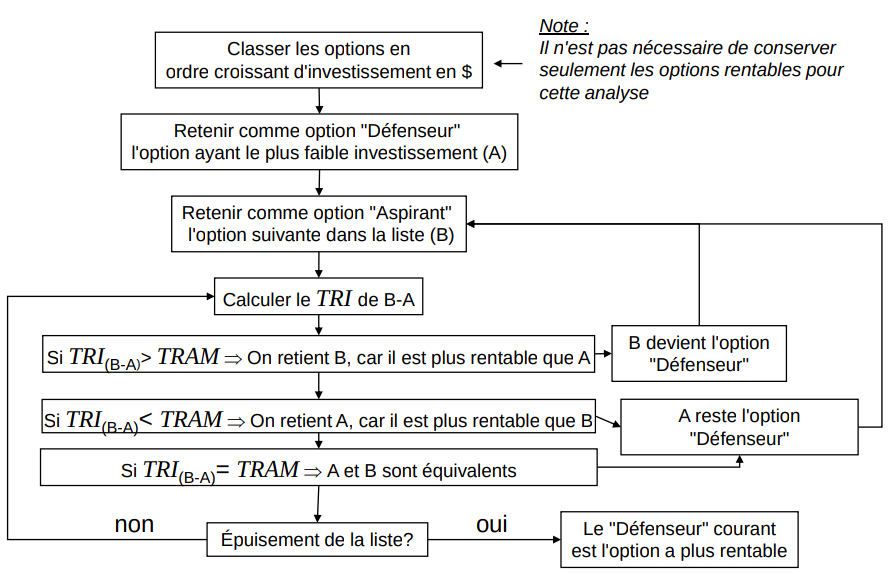
\includegraphics[scale=0.5]{images/analyse_differentielle.png}